\section{DSAM与RDDS的时间信息}\label{sec:5-8}

在从微观能级结构向电磁约化跃迁几率 $B(XL)$ 反演的因果链中（第~5.9~节），激发能级的平均寿命 $\tau$ 构成了最为关键的时间标尺。跃迁率与寿命之间满足基本的反比关系 $\lambda_{\mathrm{tot}} = 1/\tau$；若无法精确测定激发能级的微观寿命，仅凭相对分支比与角分布无法解耦出绝对的微观跃迁矩阵元模平方。

在在束 $\gamma$ 谱学实验中，皮秒（$\text{ps}$）至飞秒（$\text{fs}$）量级的超快核跃迁远远超出了常规电子学时间数字转换器（TDC）或恒比定时（CFD）通道的直接物理时间分辨率（通常约为几百皮秒至纳秒量级）。为了突破这一硬件时间测量极限，现代实验谱学普遍利用核反应产生的高速反冲核在真空飞行或固体介质慢化过程中产生的时间--空间多普勒频移特征，分别发展了反冲距离多普勒频移法（Recoil Distance Doppler-Shift, RDDS）以及多普勒频移衰减法（Doppler Shift Attenuation Method, DSAM）~\cite{dewald-2012-ddcm-recoil-distance, book-wu-nuclear-experiment-methods}。

若对多普勒几何变换、减速介质阻止本领（Stopping Power）模型、微分衰变曲线法（DDCM）以及侧向馈入时间卷积缺乏清晰界定，极易在寿命反演中引入显著的系统性偏置：例如混淆静止系发射角与实验室观测角导致多普勒频移计算失真，在直接符合门中错误将飞行发射假定为离靶瞬间布居，或者在减速截面存在理论不确定度时低估 DSAM 寿命误差。本节从相对论多普勒几何出发，推导 RDDS 的飞行时间映射与 DDCM 解析方程，系统剖析 DSAM 谱形展宽的连续慢化与停止截面机制，界定各测时技术的敏感窗口与适用边界，为第~5.9~节绝对跃迁强度的精确提取提供可追溯的时间信息基础。

\subsection{多普勒效应与相对论变换几何}\label{subsec:5-8-1}

考虑在核反应中获得反冲初速度 $\mathbf{v}$ 的激发态残核，其在实验室参考系中相对光速的比值为 $\boldsymbol{\beta} = \mathbf{v}/c$，对应的相对论 Lorentz 因子为 $\gamma = 1/\sqrt{1 - \beta^2}$。设该原子核在其静止参考系中退激发射一个固有能量为 $E_0$ 的单色 $\gamma$ 光子。

在实验室参考系中，探测器位于相对于反冲速度矢量夹角为 $\theta_{\mathrm{lab}}$ 的方向。由四维波矢量的标准 Lorentz 变换，实验室系测得的光子能量 $E_{\mathrm{obs}}$ 满足相对论多普勒频移公式~\cite{dewald-2012-ddcm-recoil-distance}：
\begin{equation}\label{eq:5-8-doppler-rel}
E_{\mathrm{obs}} = \frac{E_0}{\gamma (1 - \beta \cos\theta_{\mathrm{lab}})}.
\end{equation}
在此必须注意角动量变换几何：式~\eqref{eq:5-8-doppler-rel} 中的极角 $\theta_{\mathrm{lab}}$ 是实验室系中的实际观测角度，不可将其与原子核静止系中的发射角 $\theta_{\mathrm{rest}}$ 相混淆（二者满足相对论光行差关系 $\cos\theta_{\mathrm{rest}} = \frac{\cos\theta_{\mathrm{lab}} - \beta}{1 - \beta\cos\theta_{\mathrm{lab}}}$）。

在典型的低能核结构重离子熔合反应中，反冲核速度通常较小（典型范围为 $\beta \sim 1\%$–$3\%$）。在低速非相对论极限（$\beta \ll 1$）下，对式~\eqref{eq:5-8-doppler-rel} 按 $\beta$ 进行一阶展开：
\begin{equation}\label{eq:5-8-doppler-approx}
E_{\mathrm{obs}} \approx E_0 (1 + \beta \cos\theta_{\mathrm{lab}}).
\end{equation}
低速近似下，探测器在前进方向（$\theta_{\mathrm{lab}} = 0^\circ$）测得最大蓝移能量 $E_{\max} \approx E_0 (1 + \beta)$，在后退方向（$\theta_{\mathrm{lab}} = 180^\circ$）测得最大红移能量 $E_{\min} \approx E_0 (1 - \beta)$，而在垂直方向（$\theta_{\mathrm{lab}} = 90^\circ$）一阶多普勒频移消失，仅残留二阶横向多普勒红移 $E_{\mathrm{obs}} = E_0/\gamma \approx E_0 (1 - \frac{1}{2}\beta^2)$。

在时间单位与时钟参考系上，设 $\tau$ 为激发态在原子核自身静止参考系中的本征平均寿命。由相对论时间膨胀，若反冲核具有运动速度矢量 $\mathbf{v}(t)$，在实验室时间 $t$ 内原子核经历的本征时间积分为：
\begin{equation}\label{eq:5-8-proper-time-integral}
s(t) = \int_0^t \frac{\mathrm{d}t'}{\gamma(t')}.
\end{equation}
在实验室时间中发射光子的概率密度满足：
\begin{equation}\label{eq:5-8-lab-decay-density}
w(t) = \frac{\exp\left(-s(t)/\tau\right)}{\gamma(t) \tau}.
\end{equation}
在低速非相对论近似（$\beta \ll 1$，$\gamma - 1 \approx \frac{1}{2}\beta^2 \ll 1$）下，$\gamma(t) \approx 1$，$s(t) \approx t$，实验室时间下的衰变概率密度退化为标准指数形式 $w(t) \approx \frac{1}{\tau} e^{-t/\tau}$。本能级平均寿命 $\tau$ 与半衰期满足严格转换关系 $T_{1/2} = \tau \ln 2 \approx 0.69315\,\tau$。后续凡涉及核态衰变指数律均以 $e^{-t/\tau}$ 表述。

\subsection{反冲距离多普勒频移法（RDDS）与微分衰变曲线法（DDCM）}\label{subsec:5-8-2}

反冲距离多普勒频移法（RDDS）通常利用高精度的柱塞装置（Plunger）实现皮秒至纳秒量级核态寿命的测定。其基本构型是在薄反应靶后方相隔一段微米级可控距离 $x$ 处，精确平行放置一块阻挡箔（Stopper）。在靶中产生的反冲核以速度 $v$ 飞出靶背，并穿过真空飞行间隙：
\begin{enumerate}
\item 若核态在飞行途中退激（飞行时间 $t < x/v$），发射的光子具有未减速的多普勒频移，在探测能谱中形成\emph{飞行峰}（Shifted Peak, 强度记为 $I_s$）；
\item 若核态未在飞行途中衰变，而是在穿入阻挡箔停滞后才退激（时间 $t \ge x/v$），发射的光子具有核静止能量 $E_0$，在能谱中形成\emph{静止峰}（Unshifted/Stopped Peak, 强度记为 $I_u$）。
\end{enumerate}

在最理想的单能级直接布居、无任何侧向或级联馈入的教学简化下，反冲核在飞行时间 $t = x/v$ 内尚未衰变的存活概率等于静止峰在总强度中所占的份额：
\begin{equation}\label{eq:5-8-rdds-ideal}
R_u(x) \equiv \frac{I_u(x)}{I_u(x) + I_s(x)} = \exp\left( - \frac{x}{v \tau} \right).
\end{equation}
式~\eqref{eq:5-8-rdds-ideal} 是一个高度理想化的解析极限，它假定飞行速度严格单一且无后发能级级联注入。

在典型的核反应退激中，目标能级往往受到上方高能级级联退激的持续馈入。为了在包含级联馈入的复杂谱图中精确提取寿命，Dewald 等人建立了微分衰变曲线法（Differential Decay Curve Method, DDCM）~\cite{dewald-2012-ddcm-recoil-distance}。考虑目标能级 $i$ 与其直接馈入能级 $k$。令 $n_i(t)$ 为时刻 $t$ 的瞬时布居数，$b_{ki}$ 为 $k$ 的全部退激中直接进入 $i$ 的分支比，$\tau_i$ 为目标能级平均寿命。在共同的事件归一与恒定飞行速度 $v$ 下，连续时间放射性级联率方程表述为（Dewald 2012 综述 PDF 第~38~页式~(19)–(21)~\cite{dewald-2012-ddcm-recoil-distance}）：
\begin{equation}\label{eq:5-8-rate-eq}
\frac{\mathrm{d}n_i(t)}{\mathrm{d}t} = -\frac{n_i(t)}{\tau_i} + \sum_k b_{ki} \frac{n_k(t)}{\tau_k}.
\end{equation}
定义时刻 $t$ 之后与之前的累计退激数分别为：
\begin{equation}\label{eq:5-8-cum-counts-def}
U_i(t) \equiv \int_t^\infty \frac{n_i(t')}{\tau_i} \mathrm{d}t', \qquad S_i(t) \equiv \int_0^t \frac{n_i(t')}{\tau_i} \mathrm{d}t'.
\end{equation}
在完整事件样本与距离无关的总体曝光归一化下，两项之和恒等于能级 $i$ 的全退激总数：$S_i(t) + U_i(t) = \int_0^\infty \frac{n_i(t')}{\tau_i}\mathrm{d}t' = \text{常数}$。因此，即使在存在级联馈入的开放级联中，$\frac{\mathrm{d}S_i}{\mathrm{d}t} = -\frac{\mathrm{d}U_i}{\mathrm{d}t}$ 依然成立。对式~\eqref{eq:5-8-rate-eq} 从 $t$ 积分至 $\infty$，假设所有相关激发态的布居在 $t\to\infty$ 时趋于零，可得瞬时布居为 $n_i(t) = U_i(t) - \sum_k b_{ki} U_k(t)$；而瞬时退激发射率为 $\frac{\mathrm{d}S_i}{\mathrm{d}t} = \frac{n_i(t)}{\tau_i}$。在反冲核速度 $v$ 恒定且满足 $t \approx x/v$ 的低速非相对论与瞬时阻止近似下，单谱或总投影谱 DDCM 寿命方程表述为：
\begin{equation}\label{eq:5-8-ddcm-singles}
\tau_i(x) = \frac{U_i(x) - \sum_k b_{ki} U_k(x)}{v \frac{\mathrm{d} S_i(x)}{\mathrm{d}x}} = \frac{U_i(x) - \sum_k b_{ki} U_k(x)}{-v \frac{\mathrm{d} U_i(x)}{\mathrm{d}x}}.
\end{equation}
式~\eqref{eq:5-8-ddcm-singles} 表明：即使由于 $S_i + U_i = \text{常数}$ 使得分母中的微分项可以通过 $\frac{\mathrm{d}S_i}{\mathrm{d}x} = -\frac{\mathrm{d}U_i}{\mathrm{d}x}$ 相互代换，分子的瞬时布居中依然\textbf{必须扣除来自上方所有已知能级的累计馈入贡献} $\sum_k b_{ki} U_k(x)$。在理想两级级联模型中，若忽略正向级联馈入项，分子未扣除多余布居将导致提取的表观寿命被系统性高估；而在包含多重旁路、复杂本底与效率随能量变化的实际测量中，馈入偏差的幅度和方向依赖于具体的级联结构与扣除模型。

为了消除复杂旁路与未分辨慢侧馈对单谱分析的干扰，实验上广泛采用符合门选技术。考虑对紧邻目标能级的直接馈入跃迁 $B$ 与目标态退激跃迁 $A$ 进行 $\gamma$-$\gamma$ 符合。若在直接馈入跃迁 $B$ 的飞行移位成分 $B_s$ 上设置符合门，则该门选出的物理事件子集满足：\emph{馈入跃迁 $B$ 在反冲核脱离反应靶后、撞击阻止箔前的飞行间隙内发射}（其初次布居时刻为发射时间 $t_B \in [0, x/v]$）。必须严格澄清：直接移位门 $B_s$ 绝非要求目标态在脱离靶时（$t=0$）就已经完全直接布居；上游核态依然可以在整个飞行间隙内的任意位置发生级联退激，只是该符合条件将未能在飞行区进入 $B$ 跃迁的旁路级联以及在靶内停滞衰变的慢成分排除了。

在门选通道纯净且符合计数具有与距离无关的统一曝光归一化的条件下，直接门选 DDCM 方程精确表述为（Dewald 等人 2012 PDF 第~40~页式~(30)–(34)~\cite{dewald-2012-ddcm-recoil-distance}）：
\begin{equation}\label{eq:5-8-ddcm-gated}
\tau_i(x) = \frac{\{B_s, A_u\}(x)}{v \frac{\mathrm{d}}{\mathrm{d}x} \{B_s, A_s\}(x)}.
\end{equation}
其中 $\{B_s, A_s\}(x)$ 与 $\{B_s, A_u\}(x)$ 分别为在距离 $x$ 处测得的双移位峰符合计数与移位--未移位符合计数。在此必须指出三点重要的数据处理边界：
\begin{enumerate}
\item \textbf{门总计数的距离依赖性与分母导数}：在门选通道中，门总计数 $I_{\mathrm{gate}}(x) \equiv \{B_s, A_s\}(x) + \{B_s, A_u\}(x)$ 随柱塞距离 $x$ 呈非减演化（在小距离敏感区随距离拉长而增大，在远距离大衰变区趋于平台）。因此在其导数非零的距离区间内，$\frac{\mathrm{d}}{\mathrm{d}x} I_{\mathrm{gate}} \ge 0$，使得 $\frac{\mathrm{d}}{\mathrm{d}x} \{B_s, A_s\}$ 与 $-\frac{\mathrm{d}}{\mathrm{d}x} \{B_s, A_u\}$ 一般不可相互替换。在式~\eqref{eq:5-8-ddcm-gated} 中，分母必须严格对飞行符合峰 $\{B_s, A_s\}$ 进行距离微分，不可随意用静止符合峰导数的负值代换。
\item \textbf{自归一化比例的禁止代入}：若在每个距离点独立除以该距离的门总计数，构造局域自归一化份额 $\widetilde{R}_u(x) = \{B_s, A_u\}/I_{\mathrm{gate}}$ 与 $\widetilde{R}_s(x) = \{B_s, A_s\}/I_{\mathrm{gate}}$，若将此相对份额直接代入式~\eqref{eq:5-8-ddcm-gated} 求导，将因漏掉 $I_{\mathrm{gate}}(x)$ 自身的距离导数项而引入严重的系统误差。
\item \textbf{间接符合门与修正因子 $\alpha(x)$}：当对更高能级的上游跃迁 $C$（经由中间未设门跃迁级联进入目标态）或具有复杂分支的通道设门时，Dewald 等人给出了间接门 DDCM 表达式：
\begin{equation}\label{eq:5-8-ddcm-indirect}
\tau_i(x) = \frac{\{C_s, A_u\}(x) - \alpha(x) \{C_s, B_u\}(x)}{v \frac{\mathrm{d}}{\mathrm{d}x} \{C_s, A_s\}(x)},
\end{equation}
其中 $\alpha(x)$ 为两级联符合强度的相对归一化比例因子：
\begin{equation}\label{eq:5-8-alpha-def}
\alpha(x) \equiv \frac{\{C_s, A_s\}(x) + \{C_s, A_u\}(x)}{\{C_s, B_s\}(x) + \{C_s, B_u\}(x)}.
\end{equation}
在实际分析中，必须在各个距离点检验 $\alpha(x)$ 的稳定性并取适用的距离平均值，以评估未观测旁路馈入与探测效率校正对寿命提取的不确定度。
\end{enumerate}

\subsection{多普勒频移衰减法（DSAM）与停止本领模型}\label{subsec:5-8-3}

对于寿命在皮秒以下（$\tau \lesssim 1\,\text{ps}$）的超快跃迁，微米级的机械位移精度无法再提供足够细致的飞行时间切割。此时广泛采用多普勒频移衰减法（DSAM）。

DSAM 采用带有厚衬底（如高纯 Au 或 Pb，厚度足以使反冲核完全停滞）的固体靶。反冲核在进入衬底介质后，在减速时间尺度内迅速慢化并停滞。设反冲核在衬底介质中的动能为 $E_k = \frac{1}{2} M v^2$，离子阻止本领定义为单位飞行路径上的能量损失率 $S(v) \equiv -\frac{\mathrm{d}E_k}{\mathrm{d}x} > 0$。由能量--动量微分链式法则：
\begin{equation}\label{eq:5-8-stopping-chain-rule}
\frac{\mathrm{d}E_k}{\mathrm{d}t} = \frac{\mathrm{d}E_k}{\mathrm{d}x} \frac{\mathrm{d}x}{\mathrm{d}t} = -S(v) v = M v \frac{\mathrm{d}v}{\mathrm{d}t}.
\end{equation}
因此，在非相对论低速近似下，反冲核在衬底介质中的连续减速运动微分方程严格为：
\begin{equation}\label{eq:5-8-velocity-history}
\frac{\mathrm{d}v}{\mathrm{d}t} = -\frac{S(v)}{M}.
\end{equation}
阻止本领 $S(v) = S_e(v) + S_n(v)$ 由两部分物理机制构成：与靶原子核外电子非弹性碰撞引起的电子阻止本领 $S_e(v)$（在高速区占主导），以及与靶原子核发生弹性库仑碰撞引起的核阻止本领 $S_n(v)$（在低速末段占主导，伴随显著的离子多重散射与角度偏折）。

为了建立严格的实验前向谱形重构框架，设包含反冲初始动能、反冲角分布及空间散射状态的变量集合为 $z$，其概率分布密度为 $p(z)$。在实验室时间 $t$ 处发射 $\gamma$ 光子的时间概率密度为 $w(t, z)$，探测系统在对应空间几何与时间的响应灵敏度权重为 $\epsilon(t, z)$。若探测器能量响应函数记为 $R(E \mid E_{\mathrm{obs}}, z)$，则在实验室测得的连续多普勒发射谱线前向卷积模型严格表述为：
\begin{equation}\label{eq:5-8-forward-lineshape-model}
Y(E) = C \int \mathrm{d}z \, p(z) \int_0^\infty \mathrm{d}t \, w(t, z) \, \epsilon(t, z) \, R\left(E \mid E_{\mathrm{obs}}(t, z), z\right),
\end{equation}
其中多普勒发射能量 $E_{\mathrm{obs}}(t, z)$ 由式~\eqref{eq:5-8-doppler-rel} 确定。对于无级联馈入的直接瞬时布居，$w(t) = e^{-s(t)/\tau} / [\gamma(t) \tau]$；在存在复杂级联馈入时，$w(t)$ 必须通过级联率方程与馈入时间历史执行时间卷积。若仅在实验设定的有限能量窗口内进行拟合，窗内积分仅代表该窗口下的几何与谱形接受率，不可将每个能量成分在窗内人为独立归一化后再行叠加。

在无级联馈入与对称探测几何的一阶近似下，传统实验常利用表观多普勒平均移动因子 $F(\tau)$ 描述质心频移程度（吴治华《原子核物理实验方法》第 15 章 §15.2，印437–439/PDF445–447的小节3，式(15.17)–(15.30)；其中印438/PDF446的式(15.26)给出 $F(\tau)$~\cite{book-wu-nuclear-experiment-methods}）：
\begin{equation}\label{eq:5-8-f-tau}
F(\tau) \equiv \frac{\langle \Delta E_{\mathrm{obs}} \rangle}{\Delta E_{\max}} \approx \frac{1}{v_0 \tau} \int_0^\infty v(t) \overline{\cos\phi(t)} \, e^{-t/\tau} \, \mathrm{d}t,
\end{equation}
其中 $\Delta E_{\max} = E_0 \beta_0 \cos\theta_{\mathrm{det}}$ 为未减速最大多普勒位移，$v_0$ 为初速度，$\overline{\cos\phi(t)}$ 描述了核散射引起的离子运动方向偏离初始束流轴的统计平均投影。必须强调，式~\eqref{eq:5-8-f-tau} 的质心公式在 $\theta_{\mathrm{det}} = 90^\circ$ 附近失效（一阶频移分母为零）；且质心积分丢失了精细谱形的多体信息，在统计量充分且微观阻止本领具备可靠标定的条件下，现代高精度谱学分析通常采用基于式~\eqref{eq:5-8-forward-lineshape-model} 的蒙特卡洛全多普勒谱形拟合，以充分利用波形展宽中的速度分布信息；而在低统计或快筛选分析中，质心频移方法依然作为重要的方法学参考。

DSAM 寿命提取的关键系统误差来源包括：
\begin{enumerate}
\item 理论阻止本领模型的不确定度：
常用的唯象计算模型（如 Ziegler SRIM/Biersack 模型或 Northcliffe-Schilling 经验表）在低速重离子区（$\beta \lesssim 1\%$）的电子与核阻止截面承载着不可忽略的模型不确定度，该不确定度将直接非线性传递至拟合寿命参数中。
\item 固体衬底微观密度与界面扩散：
蒸发沉积薄膜的实际微观晶格密度通常低于块材标准密度，界面氧化层会使初始减速轨迹发生畸变。
\item 侧向馈入时间历史的解谱重叠：
如第~5.1~节式~\eqref{eq:5-1-feeding-conv} 所述，若存在未被扣除的慢侧向馈入，馈入时间将与寿命发生强共线性重叠，导致拟合寿命被严重人为高估。
\end{enumerate}

以 A. Görgen 等人（2004）在 $^{163}\mathrm{Lu}$ 中开展的厚金衬底（$12\,\text{mg/cm}^2$）DSAM 实验为例~\cite{campaign-g07-gorgen-2004-163lu-quadrupole-moments}，作者利用 Gammasphere 阵列测定了摆动激发带的寿命。作者在论文中明确强调：其给出的寿命统计误差仅包含 $\chi^2$ 拟合协方差及不同角度阵列的离散度，并未包含阻止本领模型选择所引入的全局系统误差；且带间分支比直接外源采用了先前薄靶实验数据。这一实例充分体现了 DSAM 分析必须明确标定模型依赖边界的科学准则。

\subsection{测度敏感窗口、上下限判定与方法互补}\label{subsec:5-8-4}

为直观展示 RDDS 与 DSAM 在处理不同时间尺度核态退激时的物理响应特征，图~\ref{fig:5-8-lifetime-response} 给出了基于标准教学模型的衰变曲线与多普勒线形演化图（计算参数、脚本与图工件见附录~F 与 \texttt{lifetime-response-rdds-dsam}）。

\begin{figure}[!htbp]
\centering
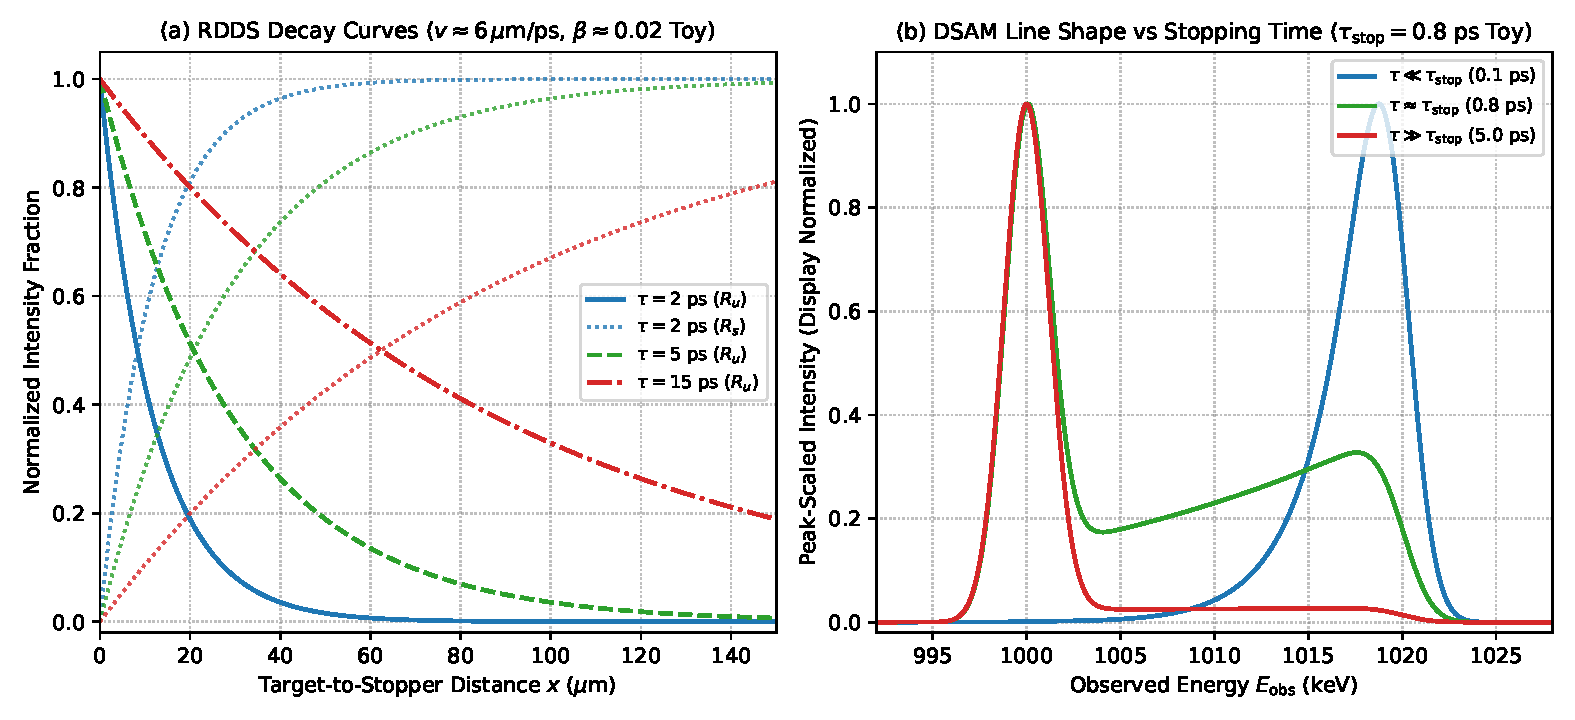
\includegraphics[width=0.98\textwidth]{Img/lifetime-response-rdds-dsam.pdf}
\caption[核态寿命测量物理响应模型对比]{核态寿命测量物理响应模型对比（规范教学示例）。(a) 展示反冲速度 $v \approx 6.0\,\mu\mathrm{m/ps}$（对应 $\beta \approx 0.02$）时，RDDS 柱塞法静止峰份额 $R_u(x)$（实线代表 $\tau = 2\text{ ps}$、虚线代表 $5\text{ ps}$、点划线代表 $15\text{ ps}$）与飞行峰份额 $R_s(x)$（点线）随靶--阻止箔距离 $x$ 的演化规律；(b) 展示厚衬底中反冲核在减速时间 $\tau_{\mathrm{stop}} = 0.8\text{ ps}$ 教学模型下的 DSAM 多普勒谱形演化：超短寿命（$\tau \ll \tau_{\mathrm{stop}}$）表现为全频移峰，中间寿命（$\tau \approx \tau_{\mathrm{stop}}$）形成连续展宽拖尾线形，超长寿命（$\tau \gg \tau_{\mathrm{stop}}$）退化为全停滞峰。计算采用解析 bin 概率与连续网格高斯卷积，在所列网格与支持域上检查总发射概率、解析质心及谱形收敛，显示图线仅将各线形峰高缩放至 1.0 以便视觉比对形态。注意此处为规范教学模型，不作为特定实验测量的修正因子。}\label{fig:5-8-lifetime-response}
\end{figure}

图~\ref{fig:5-8-lifetime-response} 阐明了核态寿命测量的敏感窗口与极限判定准则：
\begin{enumerate}
\item \textbf{DSAM 的敏感窗口与极限}：
DSAM 的测时灵敏度由核态寿命与反冲核在衬底中的慢化减速时间尺度共同决定。若核态寿命远短于离子减速至产生可辨识频移的时间，绝大多数光子将在初始高速度下发射，退化为未减速全多普勒频移峰，此时实验仅能给出寿命上限；反之，若核态寿命显著长于离子完全停滞的时间，绝大多数原子核在减速停止后才退激，主要表现为静止单色峰，此时仅能给出寿命下限。处于中间过渡寿命区间的核态则形成兼具飞行展宽与停滞峰的连续多普勒线形，其实际测时敏感范围取决于探测器能量分辨率、几何探测角度与衬底阻止特性。
\item \textbf{RDDS 的敏感窗口与互补性}：
RDDS 依赖机械位移精度（对应飞行时间 $x/v$ 从皮秒至纳秒范围）。它避免了厚衬底连续慢化谱形对微观阻止截面复杂模型的强敏感依赖，在皮秒能区与 DSAM 形成测量互补；但需要注意，反冲核穿过有限厚度反应靶与阻挡箔表层时的微小能量损失与角度散射，在精密实验中仍须进行适当建模修正。
\item \textbf{电子学快定时的延伸}：
对于几十皮秒以上乃至微秒量级的较长寿命核态，第~5.4~节讨论的高性能探测器数字时间戳差分测量与符合时间谱指数衰减曲线拟合成为主导方案。
\end{enumerate}

在科学报告中，研究人员必须根据实际实验响应，如实给出确定寿命值或无敏感性上下限，绝不能将仪器极限或理论模型假设伪造成独立的高精度测定值。由 DSAM 与 RDDS 确定的自洽寿命参量，将直接输入第~5.9~节，用于反演微观电四极跃迁几率 $B(E2)$ 与磁偶极跃迁几率 $B(M1)$。
